\documentclass[titlepage]{article}
\usepackage[utf8]{inputenc}
\usepackage{multirow}
\usepackage[table,xcdraw]{xcolor}
\usepackage{graphicx}
\title{Assignment 1}
\author{Jared See\\COP 4630 Section 2\\Professor Feng-Jen Yang}
\date{Due January 31 2023}
\begin{document}
\maketitle
{
    A Ford is a type of car. Bob owns one car. Bob parks his car at home. His house is in California, which is a state. Sacramento is the state capital of California. Cars drive on the freeway, such as Route 101 and Highway 81.
}

\subsection*{Semantic Net:}
{
    \begin{center}
        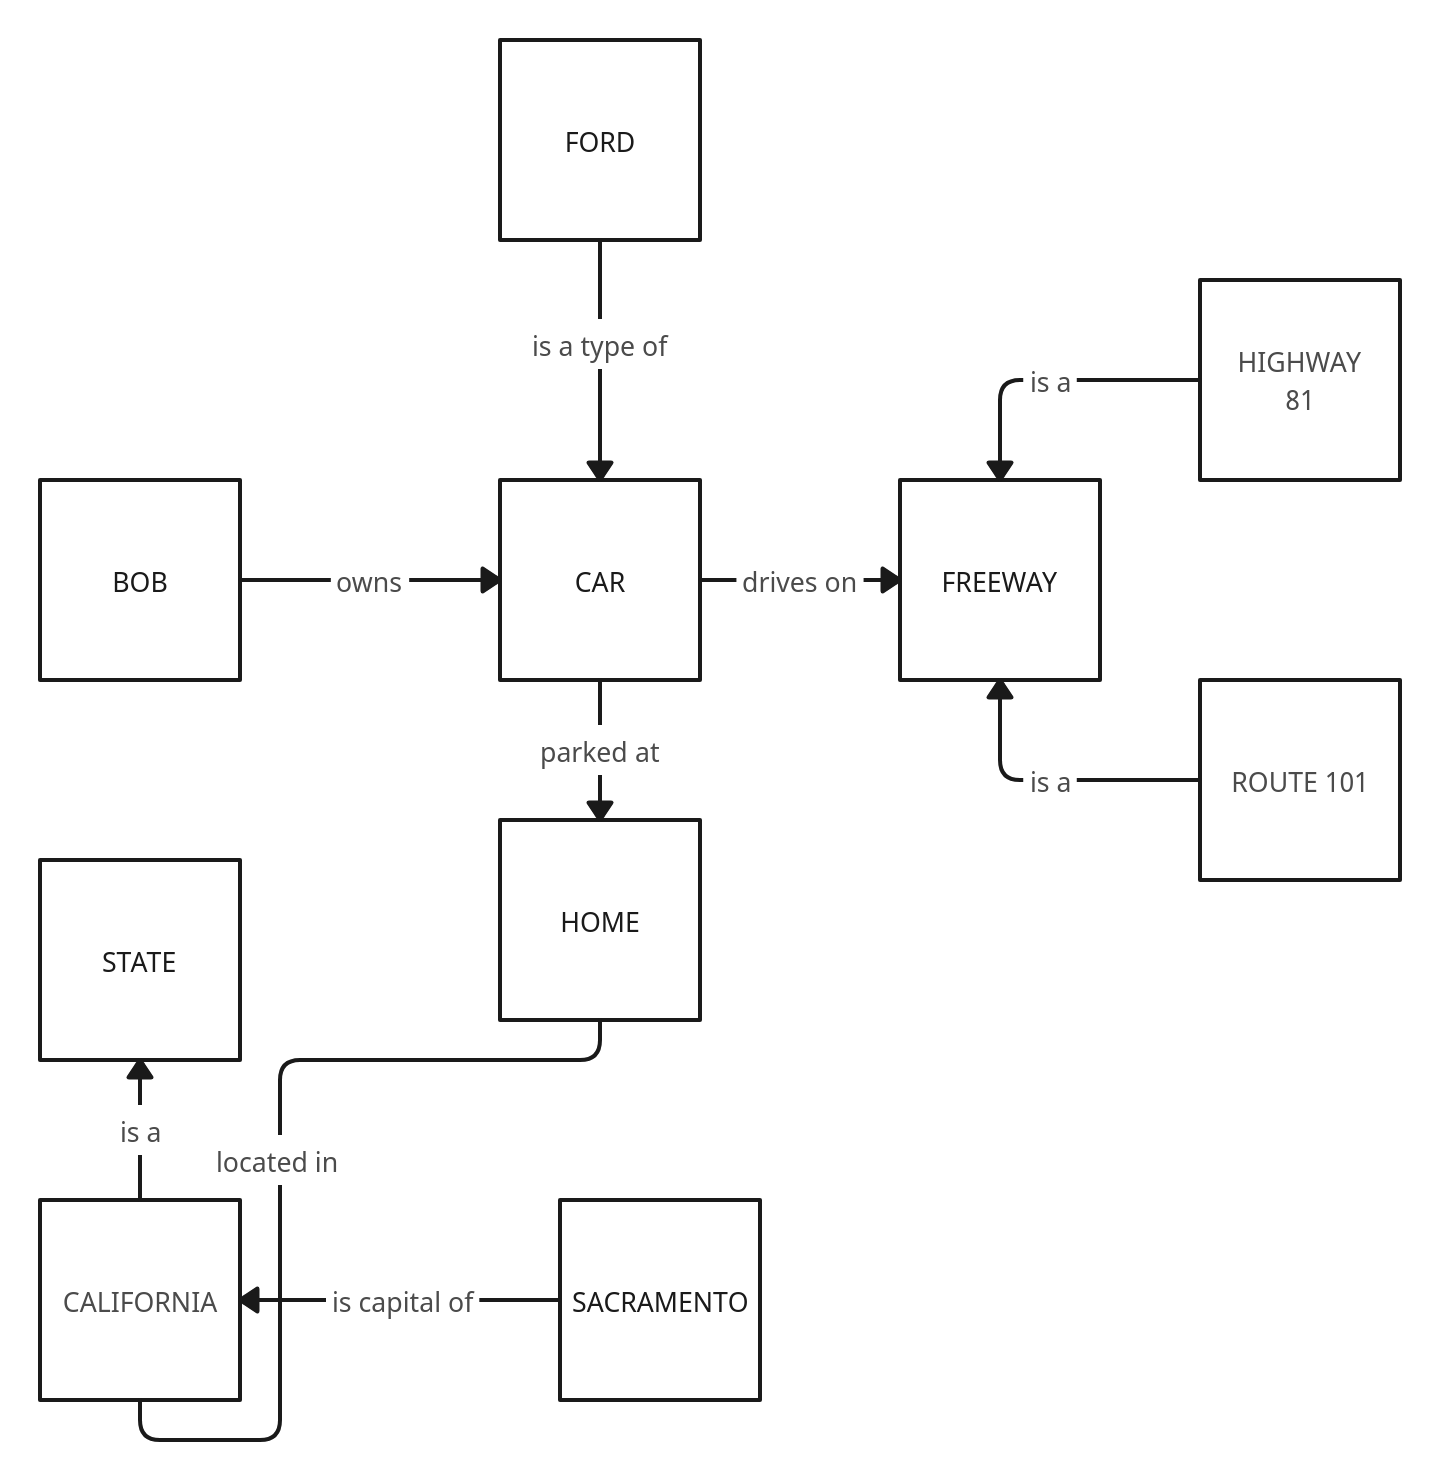
\includegraphics[scale=.2]{net.png}
    \end{center}
}


\subsection*{Frame Based:}
{
            
        % Please add the following required packages to your document preamble:
% \usepackage{multirow}
% \usepackage[table,xcdraw]{xcolor}
% If you use beamer only pass "xcolor=table" option, i.e. \documentclass[xcolor=table]{beamer}
\begin{table}[h]
\centering
\begin{tabular}{lllll}

{\color[HTML]{000000} \textbf{Frame Name}}    & {\color[HTML]{000000} \textbf{Slot}}  & {\color[HTML]{000000} \textbf{Slot Value}} &  &  \\ \cline{1-3}
\cellcolor[HTML]{C0C0C0}                      & \cellcolor[HTML]{C0C0C0}drives on     & \cellcolor[HTML]{C0C0C0}Freeway            &  &  \\
\multirow{-2}{*}{\cellcolor[HTML]{C0C0C0}Car} & \cellcolor[HTML]{C0C0C0}parked at     & \cellcolor[HTML]{C0C0C0}Home               &  &  \\
Ford                                          & is a type of                          & Car                                        &  &  \\
\cellcolor[HTML]{C0C0C0}Bob                   & \cellcolor[HTML]{C0C0C0}owns          & \cellcolor[HTML]{C0C0C0}Car                &  &  \\
Highway 81                                    & is a                                  & Freeway                                    &  &  \\
\cellcolor[HTML]{C0C0C0}Route 101             & \cellcolor[HTML]{C0C0C0}is a          & \cellcolor[HTML]{C0C0C0}Freeway            &  &  \\
California                                    & is a                                  & State                                      &  &  \\
\cellcolor[HTML]{C0C0C0}Sacrimento            & \cellcolor[HTML]{C0C0C0}is capital of & \cellcolor[HTML]{C0C0C0}California         &  & 
\end{tabular}
\end{table}
        
}



\end{document}
